\documentclass[10pt,a4paper]{article}
\usepackage[latin1]{inputenc}
\usepackage{amsmath}
\usepackage{amsfonts}
\usepackage{amssymb}
\usepackage{makeidx}
\usepackage[pdftex]{graphicx}
\author{Magni Nicol\'as, Purita Nicol\'as, Zemin Luciano R.  }
\title{Flying-High OS}
\begin{document}
\maketitle
\newpage
\tableofcontents
\clearpage

\section{Introducci\'on}
	\subsection{Objetivo}
		Se debe crear un sistema operativo multitarea, asign\'andole a cada proceso un tiempo de ejecuci\'on. El multitasker corre directamente sobre memoria y montado sobre una base de un sistema monotarea. Para cargar el Sistema Operativo se utiliza el bootloader GRUB de Unix.
	\subsection{Enunciado}
Se desea implementar un Multitasker, cuyo objetivo  principal es el de asignar tiempos de ejecuci \'on a\ diferentes procesos en memoria. El sistema deber\'a ser implementado para plataformas Intel de 32 bits, utilizando el procesador en modo protegido. El multitasker debera ser preemptivo, es decir, cualquier tarea puede ser desalojada del microprocesador. El encargado de administrar el CPU es el scheduler el cual tomar\'a como base de tiempo la interrupci\'on de hardware INT8 correspondiente al timer tick, para realizar la asignaci\'on de tiempo ( time slot ).

	\subsection{Actividades}
		\begin{enumerate}	
			\item Se deber\'a elegir la forma en que se resguardar\'a el contexto de cada tarea, y se deber\'a elejir entre las siguientes opciones
			\begin{itemize}
				\item Utilizar los TSS que provee el microprocesador Intel 386 
				\item Realizar una implementaci\'on propia de c\'odigo.
			\end{itemize}

			\item Se deber\'an implementar dos tipos de scheduling distintos. Principalmente uno de ellos deber\'a considerar la prioridad de los procesos para asignar los slots de tiempo.

			\item El sistema deber\'a estar programado de manera que se diferencien los estados b\'asicos de Corriendo, Esperando y Listo. Por otra parte, cada proceso deber \'a tener un valor de prioridad entre 0 y 4 que indique la importancia del proceso. Adem\'as se deber\'a demostrar el funcionamiento de los mismos con programas de prueba y se deber\'a poder corroborar el estado del proceso y el porcentaje de procesador que est\'a ocupando con la ayuda del comando top. Tambi\'en deber \'a existir un comando kill que permita matar procesos en ejecuci\'on. Tener en cuenta que kill debe matar tambi\'en a todos los hijos de ese proceso.

			\item Se deber\'a poder tener al menos 4 terminales distintas y alternar entre ellas de manera similar a Linux.

			\item Se deber\'an poder ejecutar diferentes tareas a trav\'es de comandos ingresados por teclado. La sintaxis de los comandos quedan a elecci\'on del desarrollador.

			\item El sistema debe tener la posibilidad de correr los mismos procesos tanto en foreground como en background. Para este \'ultimo se deber\'a utilizar el caracter \& al igual que en UNIX.

			\item El sistema debe tener un m\'odulo de administraci\'on de memoria mediante paginaci\'on para los procesos, el mismo se encargar\'a de lo siguiente:
			\begin{itemize}
				\item Cada proceso tendr\'a su stack propio en una p\'agina, a la cual solamente \'el tendr\'a acceso. Cada proceso podr\'a leer y escribir libremente sobre esta p\'agina pero no p\'aginas de otros procesos.
				\item Los procesos no poseer\'an un heap propio, ya que est\'an corriendo sobre la misma zona de datos del SO.
				\item Ningu\'n proceso deber\'a leer o escribir directamente ninguna variable global del SO. En caso de que haya variables globales que est\'en pensadas para ser leidas por procesos usuario, deber\'an tener una funci\'on que las copie a una zona de heap propia al proceso, simulando un system call.
			\end{itemize}
		\end{enumerate}

\section{Material entregado}
	Se entrega un archivo comprimido que contiene el directorio ra\'iz del proyecto. El mismo est\'a formado mediante la estructura b\'asica de un proyecto, a saber:
	\begin{itemize}
		\item inc, con todos los headers
		\item src, con el c\'odigo fuente
		\item bin, directorio de salida del kernel luego de su compilaci\'on
		\item img, directorio en donde se encuentra la im\'gen de diskette que se utilizar\'a para correr el sistema operativo, cuyo kernel se actualiza con el compilado mediante un comando en consola
		\item doc, que incluye toda la documentaci\'on del proyecto, en formato doxygen, inclu\'ido este informe
	Tambi\'en se proveen los archivos makefile, para la compilaci\'on, bochsrc, para la configuraci\'on del bochs, y mtools, para la configuraci\'on de esta utilidad.
	\end{itemize}

\section{Kernel}
	\subsection{Objetivo}
		El \textit{Kernel} es el encargado de levantar todo el sistema operativo.
	\subsection{Esquema general}
		La funci\'on principal del \textit{Kernel} es cargar en la IDT las rutinas de atenci\'on del teclado, del timer tick y las interrupciones de la \textit{int 80}, iniciar la paginaci\'on, iniciar el multitasker e inicializar las TTYs. Ademas de todas \'estas inicializaciones, tambien inicia el driver de video, el m\'odulo de shared memory, los sem\'aforos y por \'ultimo habilita las entradas del Pic que correspondan al Timer Tick y al Teclado. 
	\subsubsection{Llamadas a Sistema}
		Para inicializar cada m\'odulo se realiza una llamada a sistema, ya que en ese instante en que se esta inicializando no puede perder el procesador, por lo tanto todas estas funciones deshabilitan antes las interrupciones. Toda funci\'on que hayamos considerado que no puede perder la atenci\'on realiza una llamada a sistema.

\section{Paginaci\'on}
	\subsection{Objetivo}
		El sistema operativo debe tener un m\'odulo de paginaci\'on, por lo tanto cada proceso debe tener asociada cierta cantidad de p\'aginas. Por consecuente se debe implementar el manejo de la excepci\'on correspondiente a paginaci\'on ya que el m\'odulo de administraci\'on de memoria debe verificar que un proceso no utilize p\'aginas no asignadas a \'el. Todos los procesos comparten el heap, es decir que no existen variables globales dentro del sistema operativo, y en el caso que existiesen, deben estar en el heap del kernel, por lo tanto si el proceso desea obtener algun valor de alguna variable debe simular un system call y copiar la variables al heap propio del proceso.
	\subsection{Modelo}
	\subsection{Esquema general}
		Como se implement\'o un m\'odulo de administraci\'on de memoria, se debi\'o implemantar un \textit{malloc}. Un criterio tomado es que el kernel llama una sola vez al memory map donde obtiene todo su espacio kernel. En cambio el malloc llama reiteradas veces al memory map donde se asignan las p\'aginas asociadas al heap de ese proceso. Toda la informaci\'on de las p\'aginas asignadas se encuentran en la tabla de procesos.
	\subsection{Problemas y soluciones}
		Un gran problema que obtuvimos por medio de la paginaci\'on fue que no podiamos crear mas de 4 procesos en simult\'aneo, esto se produjo ya que luego de ver reiteradas veces el c\'odigo y no darnos cuenta de cu\'al era la causa del Page Fault, decidimos seguirlo desde c\'odigo Assembler donde pudimos encontrar la raz\'on por la que se lanzaba la excepci\'on y era porque el \textbf{CR2} ten\'ia carada una direcci\'on de una p\'agina invalida, que por lo tanto no estaba presente y lanzaba Page Fault. El principal problema fue en el armado de los frames de las p\'aginas, donde el algoritmo no contemplaba un caso donde hab\'ia que dar de baja un frame, levantar otro y asi consecutivamente. Luego de una gran reestructuraci\'on de nuestro sistema, tambie\'n nos dimos cuenta de que se nos escap\'o asignar los nuevos valores definidos en \textit{defs.h} para llevar a cabo la paginaci\'on, y por lo tanto retornaba direcciones no deseadas. Este problema se detallar\'a al final del informe.
	\subsection{Limitaciones}
		Como no se utiliz\'o segmentaci\'on de p\'aginas, el malloc siempre retorna p\'aginas contiguas y no se almacena ningun registro sobre segmentos otorgados.

\section{File System} 
	\subsection{Modelado}
		Se implment\'o una simulaci\'on de un File System, pero unicamente teni\'endose los pseudoarchivos \textit{STDIN} y \textit{STDOUT}. Cada proceso tiene almacenado en su estructura estos pseudoarchivos. Cabe destacar que nuestro sistema operativo utiliza una estructura FILE para el sistema de archivos, la cual es muy similar a la de UNIX.
	\subsection{Esquema general}
		Al tener cada proceso sus archivos de entrada y salida, result\'o f\'acil anexar los mismos a las ttys, que ser\'an explicadas luego. As\'i, ante un cambio de contexto a otro proceso, o ante un cambio de foco de tty, los procesos no pierden su posibilidad de utilizar estos archivos, a menos que realmente no deban realizarlo, en cuyo caso el sistema operativo se encarga de manejarlo.	
	\subsection{Problemas y soluciones}
		Inicialmente, los procesos no ten\'ian un filesystem propio, sino que compart\'ian un filesystem que pose\'ia cada tty. Esto trajo much\'isimos problemas en cuanto a manejo de la salida y entrada est\'andard de los procesos. Afortunadamente se resolvi\'o implementarlo de la forma antes explicada, y esto trajo muchas soluciones.
	\subsection{Limitaciones}
		Si bien la limitaci\'on m\'as obvia es que no se posee un filesystem propiamente dicho, sino que solo se tienen archivos de entrada y salida est\'andard para cada proceso, este pseudo filesystem es f\'acilmente extendible a, quiz\'as, un filesystem completo, partiendo probablemente de un archivo de salida de error, y luego un sistema de archivos propiamente dicho.
\newpage
\section{TTY}
	\subsection{Objetivo}
		Dado un numero maximo de tty's, estas son creadas en la inicializaci\'on del  sistema. Estas almacenan informaci\'on que s\'olo es modificada por la TTY, ya que esta es la encargada de traducir los distintos lenguajes que se manejan en el sistema. 
	\subsection{Modelo}
		Al comienzo del desarrollo del proyecto, no estaba claro el concepto de TTY, y por esta raz\'on se decidi\'o investigar sobre el mismo. Se decidi\'o seguir, a grandes rasgos, el modelo de UNIX, con sus respectivos ajustes. Al iniciar el sistema ,se crea una cantidad fija de tty's, all\'i se almacena toda la informaci\'on necesaria para el buen funcionamiento, y luego es seteada la tty en foco, que ser\'a modificada ante cualquier entrada o salida de datos. A cada tty se le asocia un proceso corriendo en ella, como as\'i tambi\'en son almacenados buffers de entrada y salida de datos. Respecto a los demas campos que posee su estructura, estos son utilizados para un menejo correcto de los buffers. Los mismos solamente son accedidos por la tty. En el stdin se pueden encontrar todos los caracteres ingresados por el teclado, y ser\'an almacenados en la tty en foco. Respecto al stdout de la tty, es un buffer circular de tama\~no igual al de la pantalla, y se mantiene el scroll de la pantalla, mateniendo el estado actual de la misma. En este la informaci\'on almaceanda es en lenguaje shell. Se hizo de esa forma, para que sea m\'as sencillo parsear el stdout, en el caso de querer redireccionarlo.
		El comportamiento de la tty puede variar dependiendo del tipo de comunicaci\'on que el proceso puede interpretar. En el modo \textbf{Can\'onico}, se interpretan los caracteres de control y se llama a la funci\'on que maneja el caracter ingresado(handler), si no es un caracter de control se lo almacena en el buffer interno. Al momento de interpretar que el usuario a presionado un \textbf{enter}, todos los caracteres ingresados son colocados en el stdin del proceso que se encuentra en foco en la tty en foco. 
		En el modo \textbf{Raw}, todo lo ingresado es colocado en el stdin del proceso, los \'unicos caracteres que son parseados son los \textbf{F1, F2, ...}, ya que es la \'unica manera de poder cambiar entre tty's. 
		Todo pasaje de informaci\'on del buffer de la tty hacia los stdin de los procesos se realiza mediante las primitivas write y read, para lograr as\'i mantener la circularidad de los buffers del file system.

	\subsection{Esquema general}
En esta secci\'on se explicara el flujo de informaci\'on dentro del sistema. Se comenzar\'a en modo \textbf{Raw}, un proceso intenta leer de su stdin alg\'un caracter ingresado, como el bufer se encuentra vac\'io, se duerme. Una vez que el usuario preciona una tecla, la misma es alamacenada en el buffer del teclado, el driver de teclado coloca el caracter ingresado en el stdin de la tty, esta toma el carcter, lo procesa, y si es un caracter de control se ejecuta la funci\'on asociada al mismo caracter, sino se lo coloca en el stdin de la tty que se encuentra en foco, y se procede a despertar el proceso dormido en la tty si es necesario.\\
		En el modo \textbf{Can\'onico}, a diferencia de lo explicado anteriormente, los datos son actualizados al sdtin del proceso una vez que se halla ingresado un \textbf{new line}\\
		Si un proceso quisiera escribir en pantalla, se realizan los siguientes pasos. En modo \textbf{Can\'onico}, el proceso es el encargado mediante la primitiva write de colocar los caracteres en el sdtout que le pertenece. En modo  \textbf{Raw} se utiliza una api encargada de colocar en pantalla los caracteres, esta api ha sido dise\~nada inspirada en \textbf{ncurses}. Ambos sdtouts son actualizados en cada interrupci\'on del timer tick, al igual que la pantalla.\\
		 
		En la figura 1 se muestra el flujo de datos, entre los drivers y la tty. En la figura 2 se muestra el flujo de datos entre los procesos y la tty. \\
	\begin{figure}
	\begin{center} 
	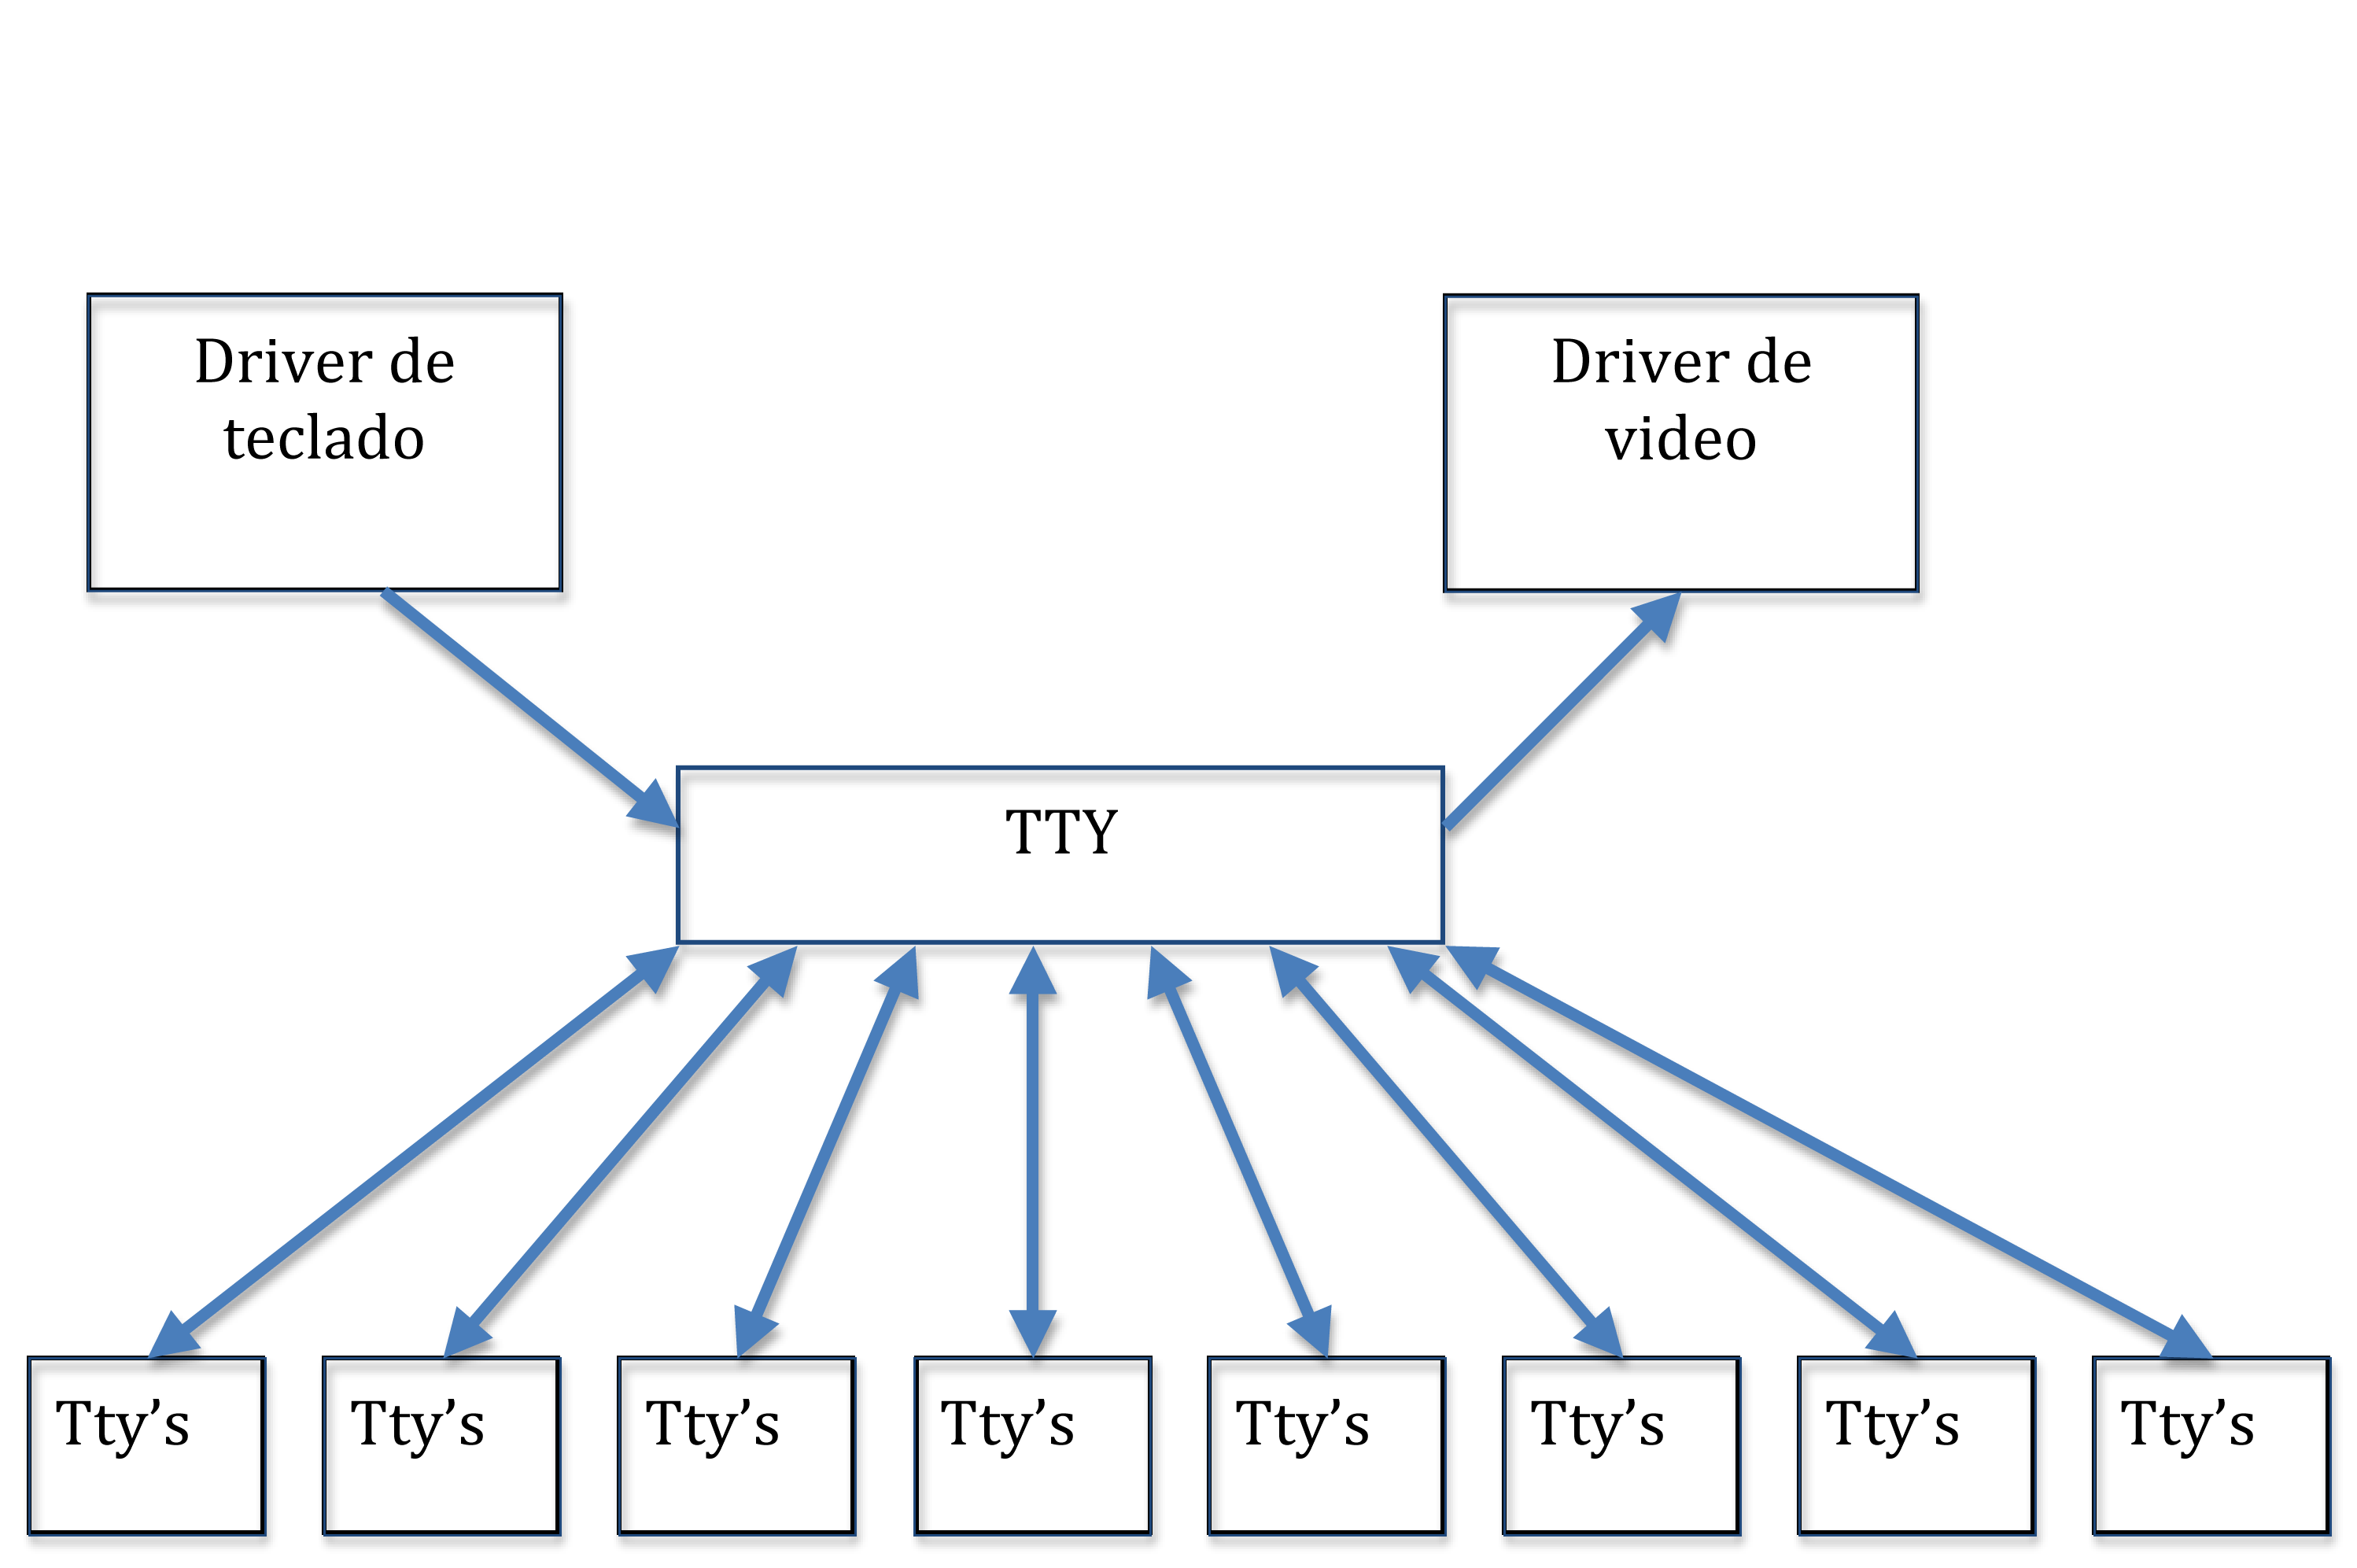
\includegraphics[angle=0, width=1\textwidth , height=0.3\textheight]{flujoTTY.png} 
	\caption{ Flujo de datos entre los driver, y la tty. }
	\end{center} 
	\end{figure}
	
	\begin{figure}
	\begin{center} 
	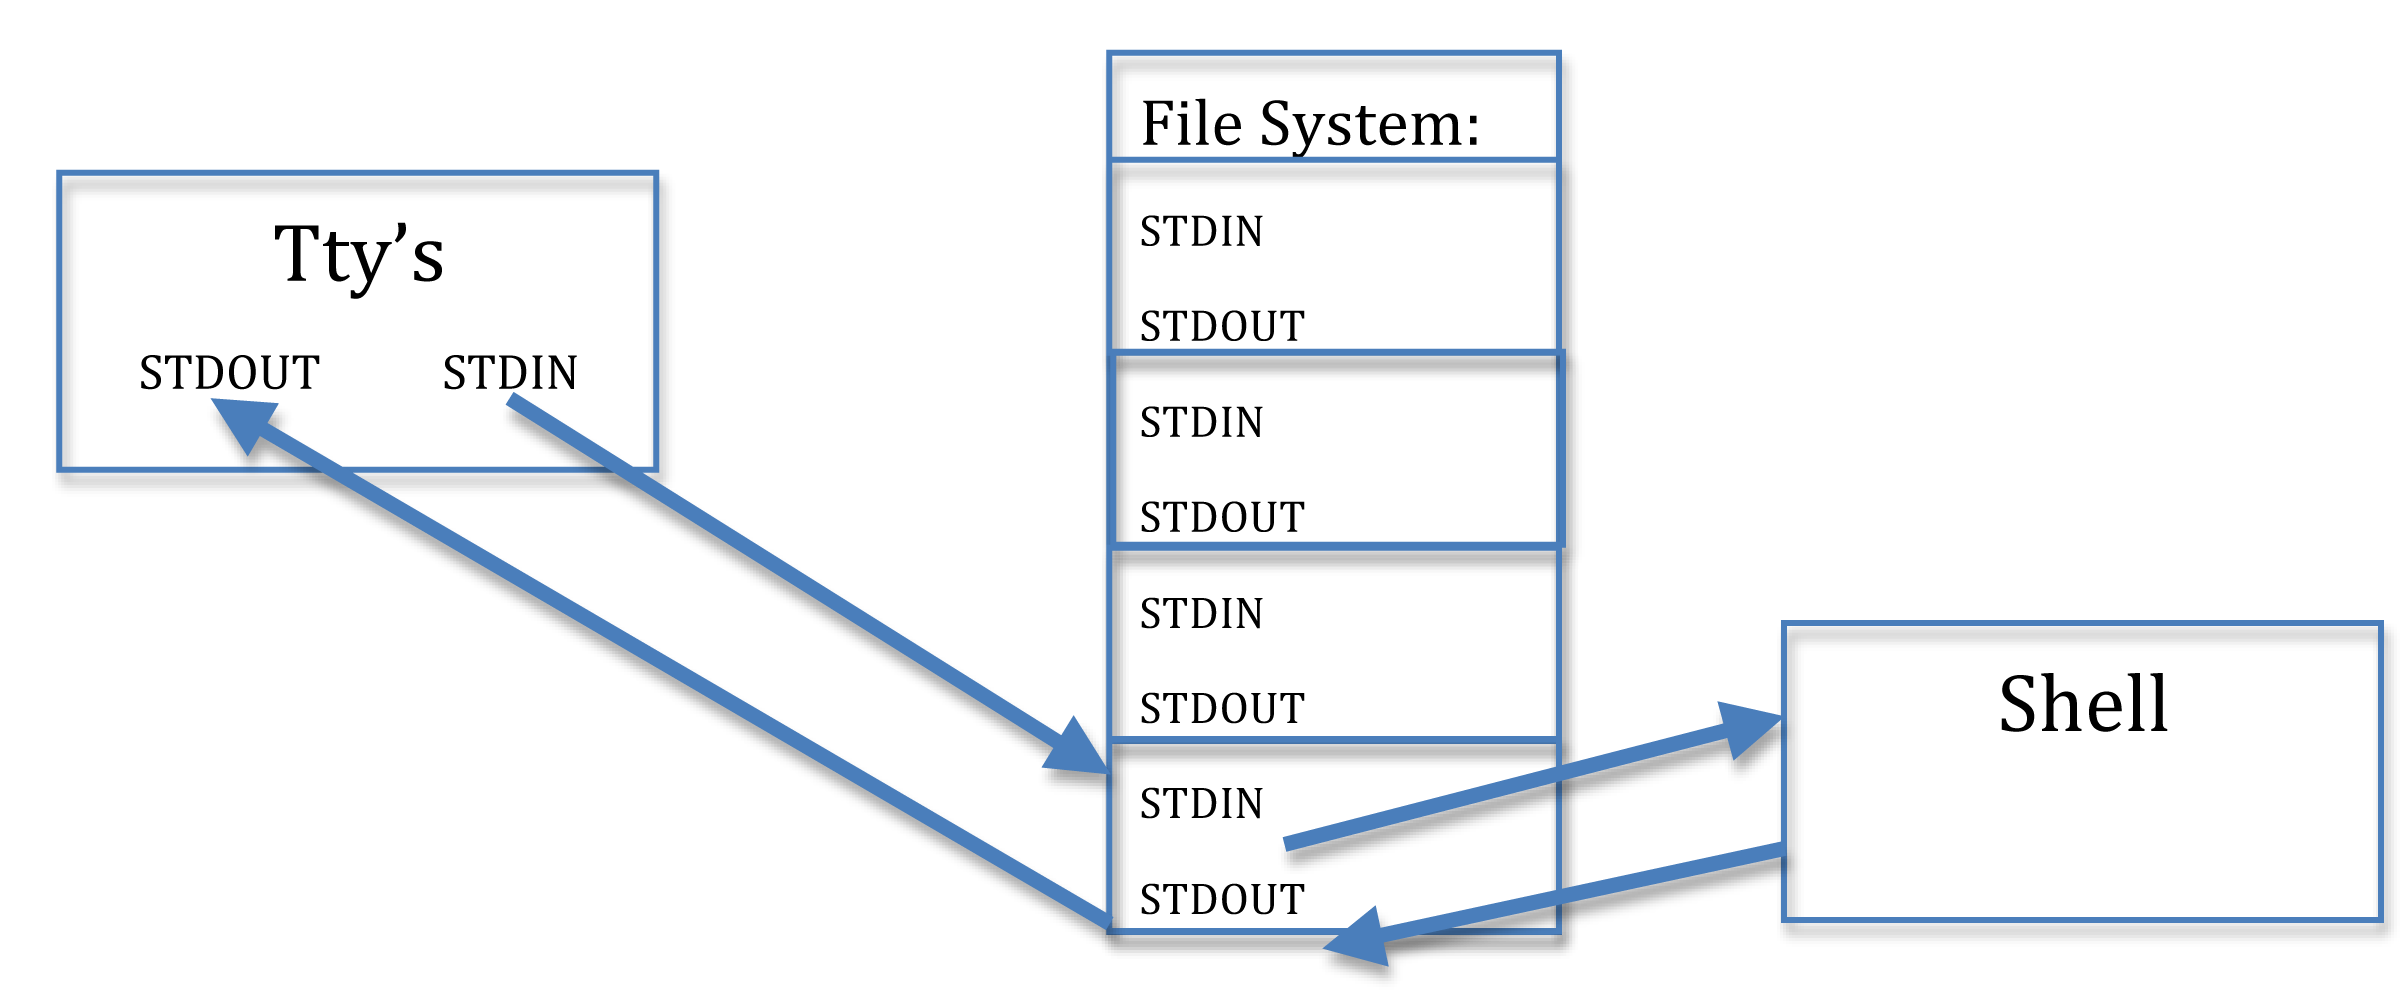
\includegraphics[angle=0, width=1\textwidth , height=0.3\textheight]{flujoTTY2.png} 
	\caption{Flugo de datos entre los procesos, la tty y el stdout}
	\end{center} 
	\end{figure}

	\subsection{Problemas y soluciones}
		Se nos presentaron muchos problemas con la TTY ya que a medida que se iba leyendo caracteres o preguntando algo, nos d\'abamos cuenta de que ten\'iamos que mejorarlo, y, por lo tanto, las TTYs sufrieron infinidad de modificaciones desde el comienzo del desarrollo, desde su inexistencia, hasta convertirse en un sistema realmente avanzado en lo que nos respecta.\\
		El primer problema que nos surg\'io fue el de los lenguajes que manejaba la TTY, relacionado con sus buffers. En un principio ten\'iamos un \'unico \textit{STDIN}, por lo que tuvimos que cambiarlo y asignarles un buffer \textit{STDIN} a cada TTY. \\
		Otro problema con \'esto fu\'e la diferenciaci\'on entre el \textit{STDIN} y \textit{stdin}, donde para nosotros el \textit{stdin} es la entrada est\'andar del proceso que estaba corriendo y no necesariamente es el que est\'a en foco en la TTY actual, menos a\'un podr\'ia serlo si fuera una shell que se encuentra dormida. Por lo tanto se tuvieron que modificar los write y read para que escriban sobre un \textit{stdin} y \textit{stdout} indicado, implement\'andose para ello las funciones fread y fwrite. Cabe destacar que nos result\'o bastante complicado darnos cuenta de que ante un pasaje de datos desde la tty hacia el proceso correspondiente que colgaba de la misma, en realidad se le estaba pasando la informaci\'on al proceso que estuviera corriendo al momento que el timer tick interrump\'ia, y a su vez resolver escribir en el proceso que se encontraba en foco en la tty en foco, valga la redundancia. Este problema surg\'ia ante un enter, ya que la linea que la tty acababa de procesar deb\'ia ser entregada al proceso que correspondiera, el cual ser\'ia el proceso en foco en la tty en foco, como se dijo antes. El problema era que en la funcion que se encargaba de eso, se utilizaba un write en STDIN, y para nosotros, stdin es el stdin del proceso que est\'a corriendo, que no necesariamente es el que esta en foco en la tty actual. Menos a\'un podr\'ia serlo si es una shell que est\'a dormida. Por ese motivo, se tuvo que implementar una funci\'on que devolviera el stdin del proceso en foco en la tty en foco para asi poder darle la informacion, mediante las mencionadas fread y fwrite.
		Un problema de no gran envergadura fue el manejo de los \'indices, ya que en un principio se utilizaron dos variables de desplazamiento \'unicamente, y se incrementaba de a un paso o en el caso que fuese un caracter de control se desplazaba lo indicado por ese caracter, pero por cuestiones de simplicidad se decidi\'o utilizar una varible que indica la cantidad de caracteres que escribi\'o en el \textit{STDOUT} de la TTY, una variable que dice la fila en la cual se encuentra y una variable para la columna. Del mismo modo para las variables de lectura, se continu\'o el mismo criterio.
	\subsection{Limitaciones}
		Se tuvieron que tomar ciertas consideraciones para poder desarrollar el sistema, una de ellas es una limitada catidad de caracteres que se pueden almacenar en modo Raw, debido a que si no se presiona \textbf{new line}, el buffer de la tty no es refresacado, por esa razon se perder\'ian los caracteres ingresados una vez que el buffer est\'e completo.
\section{Procesos}
	\subsection{Objetivo}
	Se lanzar\'an inicialmente nueve procesos, y ser\'an creados en el siguiente orden, init, shell1, shell2, ... ,shell8. En la figura 3, se presenta un diagrama de arbol, demostrando la relaci\'on entre ellos. Al comenzar a correr init, este crea las 8 shells y se dueme en espera del retorno de sus hijos, tomando el procesador \'unicamente cuando no existe otro proceso en condiciones de tomarlo, como por ejemplo, si solo se encuentran creadas las 8 shells que se encuentran bloqueadas esperando datos de entrada.
	\subsection{Modelado}
	A diferecncia de linux, los procesos corren el mismo archivo binario, por esa razon se debe tener mucho cuidado con las variables globales. Cada proceso al ser creado obtiene 3 frames de paginas, que luego ser\'an utilizado para su stack y heap, tomando serias precauciones en cuanto al crecimiento de ambos, de manera que no se pisen entre s\'i. 
	\subsection{Esquema general}
	A continuaci\'on en la figura 3,  se muestra un diagrama del estado inicial del sistema una vez completada la inicializaci\'on. En la figura 4, se puede ver qu\'e pasar\'ia si el usuario quisiera ejecutar el proceso top.
	
		\begin{figure}
	\begin{center} 
	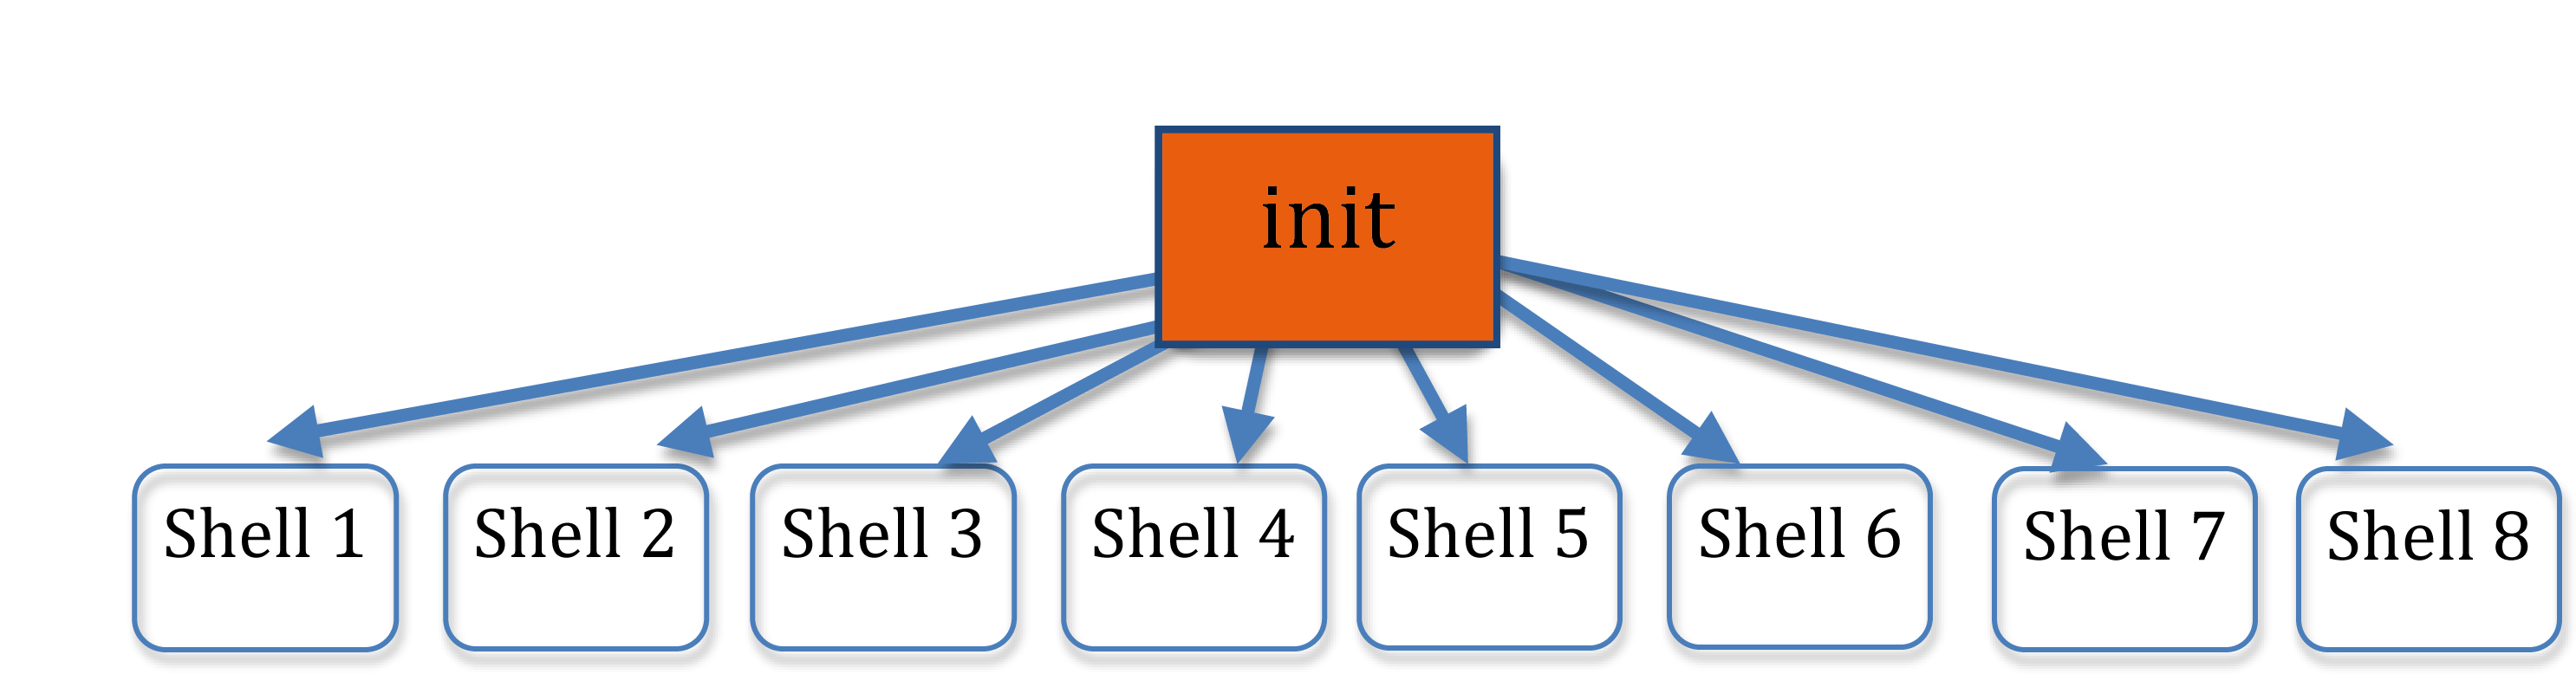
\includegraphics[angle=0, width=1\textwidth ]{procesos.png} 
	\caption{ Estado inicial del sistema, los procesos que est\'an en azul est\'an bloqueados, y los que est\'an en naraja esperan a que terminen sus hijos. El sentido de las flechas representa a qui\'en se est\'a esperando }
	\end{center} 
	\end{figure}
	
	\begin{figure}
	\begin{center} 
	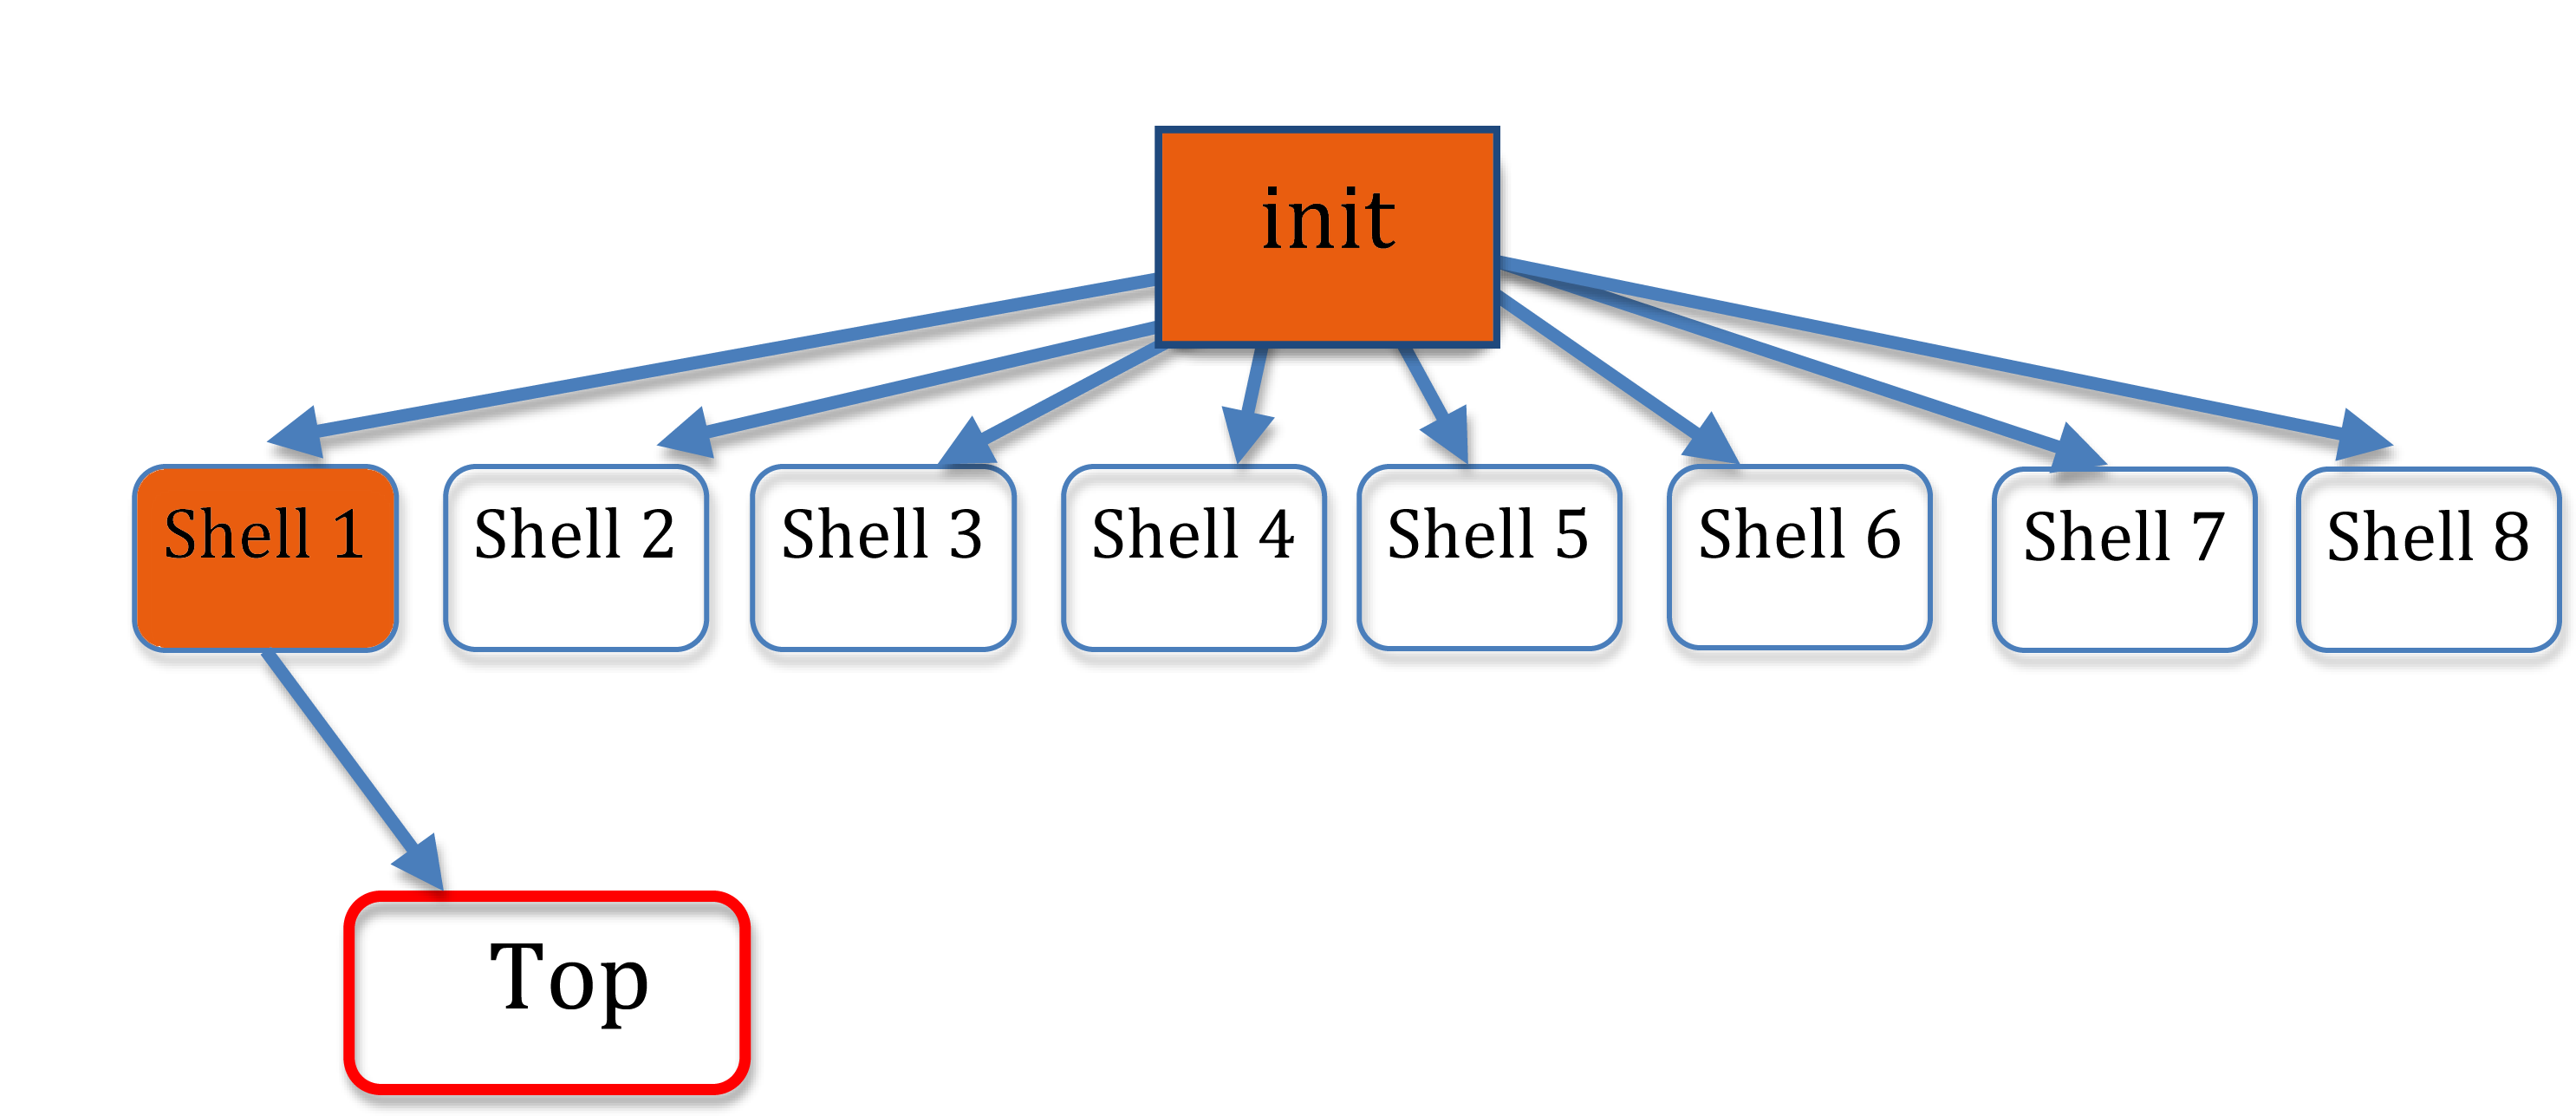
\includegraphics[angle=0, width=1\textwidth ]{proceso2.png} 
	\caption{Estado inicial del sistema, los procesos que estan en azul est\'an bloqueados, y los que est\'an en naraja esperan a que terminen sus hijos, y rojo el proceso que se est\'a ejecutando. El sentido de las flechas representa a qui\'en se est\'a esperando}
	\end{center} 
	\end{figure}
	\subsection{Problemas y soluciones}
		En \'este \'area nos topamos con 2 problemas importantes El primero fu\'e c\'omo resolver la entrega del microprocesador de manera tal que el proceso init s\'olo trabajase cuando ning\'un otro proceso pudiera hacerlo. Para ello se resolvi\'o que el scheduler retorne en dichos casos al proceso init, y que el mismo se encuentre, luego de realizar sus tareas pertinentes, en un loop "infinito" que espera a la terminaci\'on de sus hijos, y s\'olo cuando no posee nignuno, sale del loop para reiniciar el sistema, dado que en \'este punto, el control sobre el sistema ya no es recuperable.
	\subsection{Creacio\'n de procesos}
		La creaci\'on de los procesos supuso uno de los, si es que no el mayor desaf\'io del trabajo pr\'actico. Crear un proceso supone infinidades de consideraciones y acciones para su correcto funcionamiento, desde el seteo de su PID, pasando por la creaci\'on de su stack frame, hasta la asignaci\'on de su tty, la cual particularmente se hereda de su padre.
		Para todo esto, se defini\'o una estructura enorme que contiene todo lo que un proceso necesita. Esta estructura puede ser consultada en la documentaci\'on Doxygen del sistema operativo, proporcionada junto con toda la documentaci\'on.
		Para que el lector posea un panorama general, esta estructura contiene informaci\'on acerca del pid del proceso, el pid de su padre, el filesystem del proceso, su nombre, sus frames de heap y stack, su prioridad, la cu\'al es utilizada por el scheduler, la informaci\'on de los hijos del proceso, su estado de atomicidad, su estado respecto al sistema, que puede ser, entre otras cosas, bloqueado, corriendo o listo, la tty que tiene asignada, y su nivel respecto de la tty que posee asignada, que puede ser background o foreground.
		El armado del stack frame de los procesos supuso la mayor complicaci\'on del procedimiento de creaci\'on de los mismos. Dado que en nuestra forma de cambio de contexto, se "enga\~n a" al microprocesador para que "retorne" de la interrupci\'on del timer tick al siguiente proceso, el stack frame debe contener los datos necesarios para que este retorno de interrupci\'on funcione correctamente, y por encima de dichos datos, la informaci\'on pertinente del proceso en s\'i.
		El mayor problema fu\'e la confecci\'on y de los punteros esp y ebp, que pasar\'ian a ser los del proceso siguiente, ya que deber\'ian estar construidos de manera tal que al retornar del multitasker, el stack se recuperase correctamente de los movimientos que hab\'ia realizado antes de cambiar el contexto, y as\'i luego del retorno, en el handler de la interrupci\'on, al realizar el pop de los registros backupeados y realizar iret, el microprocesador tomase como direcci\'on de retorno, segmento de c\'odigo e eflags, los correspondientes al comienzo del proceso elegido.
		Otro problema creando el stack frame fue que inicialmente utiliz\'abamos en compilaci\'on la opci\'on -O para optimizaci\'on, el compilador en la funci\'on del multitasker hacia una compilaci\'on in-line de una funci\'on que utiliza la misma, llamada freeterminatedproceses, la cual requer\'ia 3 registros para trabajar, y adem\'as un espacio para variables locales mayor. Debdio a eso, el compilador para la funci\'on multitasker reservaba un tama\~o para las mismas mucho mayor que el est\'andard de 0x000018, y por ello, cuando uno arma el stock frame, en el esp tiene que reservar dicho tama\~o para que cuando en el multitasker se cambie el stock, al salir la funci\'on, la misma acomode el stack pointer adecuadamente para que obtenga la direcci\'on de retorno correcta, y as\'i poder luego en el handler de la int-08 con el iret "retornar" al nuevo proceso seleccionado por el multitasker. Para solucionar esto, se realiz\'o un seguimiento l\'inea a l\'inea de la salida de assembler de la compilaci\'on de la funci\'on del multitasker, y as\'i se encontr\'o esta compilaci\'on in-line, y luego se la desactiv\'o para verificar que solo se reservara 0x000018, y poder as\'i definir el tama\~o para variables locales de esa forma, y poder armar correctamente el stack frame.
	\subsection{Herencia de TTY's}
		La herencia de ttys, si bien no result\'o complicada, merece cierta menci\'on. Inicialmente, los procesos no poseen una tty asignada. Pero en caso de que su padre s\'i la posea, estos heredan la misma. Para ello, inicialmente cuando init, que no posee una tty asignada, al momento de crear los procesos shell, les asigna a cada uno su tty mediante un system call, y a partir de all\'i, cualquier proceso creado por las shells hereda su tty, y as\'i sucesivamente.
	\subsection{Muerte de un proceso}
	Al terminar un proceso, este ejecuta una funci\'on gen\'erica "exit". En la misma, b\'asicamente, el proceso pasa a tener un estado TERMINATED, y fuerza la interrupci\'on de timer tick que invoca al multitasker. El mismo, luego de cambiar los procesos, siempre ejecuta una funci\'on que se encarga de limpiar los procesos que entre corrida y corrida del mismo, pudieran haber terminado, y es as\'i como los limpia.
	Dicha funci\'on exit tuvo que ser incrustada en el stack frame que se generaba al crear cada proceso.
	\subsection{Procesos ejecutados en background}
		Los procesos ejecutados en background, funcionan de la misma manera que los de foreground, excepto por el hecho de que su entrada est\'andard no es funcional, pudiendo s\'olo imprimir en pantalla mediante su stdout, tal y como sucede en UNIX.
	\subsection{Procesos especiales}
	\subsubsection{Top}
		El proceso Top es el encargado de mostrar al usuario toda la informaci\'on pertinente relacionada con los procesos que se est\'an ejecutando, desde su pid y su nombre, hasta su estado, pasando por el consumo de CPU que suponen, y su consumo de memoria, entre otras cosas. A medida que se proced\'ia con la implementaci\'on del mismo, nuevas ideas respecto de los datos que pod\'ian ser mostrados, iban vieniendo a nuestras mentes, dado que poco a poco nos d\'abamos cuenta de las posibilidades que pose\'iamos para mostrar informaci\'on, dado que la estructura de cada proceso posee mucha informaci\'on importante. 
	\subsubsection{Shell}
	En esta secci\'on se hablar\'a acerca de como fu\'e adaptada la shell para poder funcionar en un sistema multi tarea. \\ 
	Como la shell que se tom\'o como base fue dise\~nada para correr en un sistema multi tarea, se tuvieron que realizar ciertas adaptaciones. Una de ellas fu\'e, que las variables globales deber\'ian pertenecer s\'olamente a esa shell, por esa raz\'on se realiz\'o un vector donde fueron almacenadas estructuras con todos los datos pertinentes para el correcto funcionamiento de la shell. Cada shell almacenaba en su heap dichas estructuras, y \'esto asegura un nivel m\'as de seguridad, ya que una shell no podr\'a acceder a datos de otra, por que no estar\'ian presentes las paginas de la misma. \\
	En ella se implementaron procesos de prueba que se pueden ejecutar para testear la funcionalidad del sistema.

	\subsection{Problemas y soluciones}
		La clave en el desarrollo del proceso Top se encontr\'o en el c\'omputo del consumo del CPU. Para ello, cada proceso posee en su entrada de la tabla de procesos, un campo que supone un conteo de timer ticks durante los cuales recibi\'o el procesador. Los mismos son utilizados por el proceso top, mediante system calls, para computar un promedio de utilizaci\'on en porcentaje del CPU. Dichos valores son reseteados entre vuelta y vuelta del proceso top, a modo de poder ir actualiz\'andolos.
	\subsection{Limitaciones}
		Por cuestiones del algoritmo que computa la informaci\'on del consumo del CPU, el proceso Top s\'olo puede estar corriendo en una s\'ola tty.
\newpage
\section{Multitasker}
	\subsection{Objetivo}
	Intercambiar tareas mediante software, y una correcta construcci\'ion del stack frame.
	\subsection{Modelo}
		El multitasker salvar\'a el contexto de la tarea actual, apagar\'a la presencia de sus p\'aginas, cargar\'a el contexto del siguiente proceso, previo encendido de la presencia de sus p\'aginas.
	\subsection{Esquema general}
		Si bien el trabajo del multitasker no es demasiado complicado, s\'i lo es la creaci\'on del stack frame de modo que este cambio de contexto se realice correctamente, pero eso es un punto que ya ha sido tratado anteriormente.
	\subsection{Problemas y soluciones}
		Un gran problema que se tuvo con el algoritmo del scheduler fue que, al momento de cambiar los contextos, si el scheduler devolv\'ia al proceso init, debido a que no se ten\'ia otro proceso para correr, si el proceso al cual se le est\'a por quitar el procesador se encuentra en condiciones de seguir ejecut\'andose, se le otorga el procesador al mismo nuevamente, sin realizar el cambio de contexto. Esto pudo realizarse mediante una simple comprobaci\'on luego del retorno del scheduler, pero notar esa comprobaci\'on tom\'o varias horas de an\'alisis del algoritmo del mulstitasker.
\newpage
\section{Scheduler}
	\subsection{RPG}
	\subsubsection{Modelo}
		Implementar un algoritmo basado en juegos RPG. El algoritmo consite en asignarle un puntaje a un proceso en cada llamado del scheduler. Cuando un proceso llega al puntaje designado como m\'aximo se lo agrega a la lista de procesos listos para ejecutar. Luego se verifica qu\'e proceso es el que tiene m\'as antiguedad. Una vez devuelto el proceso a procesar, se reinicia el contador de puntos rpg y la antiguedad.
	\subsubsection{Problemas y soluciones}
		Principalmente tuvimos un problema manejando la antiguedad de los procesos, luego decidimos tomar una funci\'on de evaluaci\'on que nos permite ir pasando por todos los procesos, que no alcanzen inmediatamente el puntaje m\'aximo de rpg, para luego ser atendido.
	\subsubsection{Limitaciones}
		La funci\'on de evaluaci\'on en el caso de que se aumente la cantidad de procesos o disminuya habr\'ia que cambiarla, porque es en funci\'on de prioridades y cantidad m\'axima de procesos. Tambien habr\'ia que modificar el puntaje m\'aximo de rpg a alcanzar.

\subsection{Round-Robin}
	\subsubsection{Objetivo}
		Implementar un algoritmo del tipo Round Robin. B\'asicamente se comporta como una lista circular donde se van devolviendo todos los procesos que esten en estado \textbf{READY} en el orden que se encuentran en la tabla de procesos.
	\subsubsection{Modelo}
		El modelo tomado es el siguiente. Se toma la lista de procesos y se la recorre en forma lineal verificando si algun proceso se encuentra listo para ser atendido, en el caso de que haya alguno se lo devuelvo y en la pr\'oxima llamada se arranca a recorrer desde esa posici\'on y se realiza el mismo recorrido ya explicado anteriormente.
	\subsubsection{Problemas y soluciones}
		En un principio el algoritmo se quedaba en un loop infinito ya que buscasa desde init y como siempre estaba listo lo devolvia y a veces no retornaba o era interrumpido. Por lo tanto una soluci\'on fue llamar al scheduler en caso de que haya algun proceso para correr distinto de init. En un principio ten\'iamos problemas con el algoritmo porque compilabamos con la opci\'on de optimizaci\'on y se agregaban funciones en el c\'odigo que no queriamos, luego de darnos cuenta de ese error, comenz\'o a funcionar el algoritmo.
		En la recta final del desarrollo del sistema operativo, una vez implementado el m\'etodo mediante el cual el proceso init s\'olo recibe el procesador cuando ning\'un otro proceso puede recibirlo, el algoritmo de round robin comenz\'o a fallar. Simplemente no retornaba el proceso init en los casos que deb\'ia. Para ello, se revis\'o detalladamente, ahora con mayores conocimientos acerca de lo que realmente deb\'ia hacer, y se encontraron algunos errores en el mismo, que pudieron facilmente ser subsanados.
	\subsubsection{Limitaciones}
		El algoritmo en s\'i no maneja prioridades, sino el orden el cual fueron creados los procesos. Se podr\'ia hacer que la creaci\'on de procesos los inserte en forma ordenada en la tabla de procesos, y por lo tanto el algortimo \textit{Round Robin} de alguna forma estar\'ia teniendo en cuenta cierto nivel de prioridades.

\subsection{IPCs Implementaciones}
	\subsubsection{Shared memory}
		Se implement\'o un IPC basado en Shared memory, donde la cantidad de segmentos de shared memory est\'a definida por un define. Se decidi\'o utilizar la estructura que utiliza System Five para la shared memory y Posix para los sem\'aforos. Cada shared memory ya tiene asociado un sem\'aforo y la cantidad de frames que tiene desiganados para utilizar. La implementacion de shared memory y de los sem\'aforos se realiz\'o con un cuidado extremo, metodolog\'ia que se adopt\'o a partir de conocimientos obtenidos en el primer trabajo pr\'actico de la materia, que nos ense\~naron que errores \'infimos en la implementaci\'on y/o utilizaci\'on de una shared memory, desembocar\'ian en resultados desastrozos e indebuggeables. Si bien la shared memory se instancia junto con un sem\'aforo que se le provee al usuario para que controle el uso de la misma, el m\'odulo de sem\'aforos puede ser utlizado en cualquier parte y no \'unicamente para el uso de la shared memory. Los mismos fueron implementados de manera tal de que mediante un simple par\'ametro en su creaci\'on, los mismos funcionen como sem\'aforos que bloquean el uso de un recurso hasta que el mismo se libere, o como un sistema de espera hasta ser se\~nalizado por otro proceso.
	\subsubsection{Objetivo}
		Implementar un juego en donde se pueda verificar la comunicaci\'on entre procesos mediante un IPC, en nuestro caso \textbf{Shared Memory}.
	\subsubsection{Modelo}
		En un principio se decidi\'o implementar como juego un Chat entre varias shells, pero finalmente se eligi\'o hacer la batalla naval con ciertas restricciones. La creaci\'on de barcos se genera en forma aleatoria, es decir que se implement\'o un random muy b\'asico donde usa un polinomio de grado 1 y como semilla utiliza los ticks realizados por el timer tick hasta el momento desde la carga del sistema operativo. El juego es de dos personas \'unicamente, como la tradicional batalla naval.
	\subsubsection{Esquema general}
		La forma en que se nos ocurri\'o para comunicar los dos procesos es que cuando se crea ese proceso, el juego proporciona la opci\'on de ser host o unirse a una partida ya creada. Por lo tanto cuando se crea el primer proceso uno puede elegir entre ser host o unirse a una partida ya creada, y la forma de unirse es que cuando se crea el proceso host, se le muestra en pantalla el ID de la shared memory creada, por lo tanto el jugador 2 debe ingresar ese id para unirse a esa partida. Una vez ya pasados los primeros pasos comienza el juego. La informaci\'on que viaja por la shared memory son las posiciones del tablero en donde se ubicaron las bombas. En un principio se hab\'ia dicho de poner el tablero de cada jugador en la shared memory y que el jugador escribiera directamente sobre esa posici\'on, pero nos dimos cuenta que en verdad la informaci\'on que necesitan los dos son las posiciones del tablero para cada uno actualizar donde fu\'e puesta la bomba y verificar si le di\'o a algun barco o si fu\'e agua. \\
		Cada vez que un usuario ingresa una posici\'on en donde desea ubicar la bomba, se bloquea el tablero y una vez enviado el mensaje se desbloquea. De esta forma evitamos que los dos jugadores pongan en el mismo instante dos posiciones distintas y se mezclen sus ubicaciones.
	\subsubsection{Problemas y limitaciones}
		Un problema fue tomar la decisi\'on de ubicar los barcos, si el usuario los pod\'ia ubicar o si lo gener\'abamos nosotros, pero se opt\'o por la segunda y los barcos pueden estar unicamente verticales u horizontales, no diagonales. \\
		Otro problema que nos surgi\'o fue que los sem\'aforos se quedaban esperando pero se seguia imprimiendo el tablero esperando la conexi\'on de alg\'un usuario al juego, por lo tanto decidimos modificar los sem\'aforos para que se queden esperando y no pueda realizar otra cosa, entonces cuando alguien ingresa una posici\'on, reci\'en entonces se refresca el tablero.  
\newpage
\section{Otros problemas de relevancia}
	Los cli y sti, que deshabilitan interrupciones por hardware fueron tambi\'en un problema. Dado que no son anidables, al comienzo fue complicado ver donde deber\'ian utilizarse los cli y sti correspondientes para lograr una atomicidad apropiada par los manejos de interrupciones. Luego de un extenso an\'alisis, se corrobor\'o que al comienzo de un manejador de interrupci\'on, deshabitar las interrupciones mediante cli no implicaba que al retornar las mismas siguieran deshabitadas, dado que se recuperan los eflags del proceso que fue interrumpido, y en dichos eflags las interrupciones segu\'ian habilitadas. Por ello, se concluy\'o que sti no es necesario utilizarlo dado que consecutivas llamadas a interrupciones, sin retornar de la primera, no requieren de ning\'un sti dado que deben ser todas at\'omicas, y que se restituir\'ian las mismas en cuanto la primera retornase. Es por ello que Sti solo se utiliza en el modulo de arranque del kernel para poder cargar correctamente el vector de interrupciones. Los cambios de contextos por s\'i solos logran restaurar la habilitaci\'on de interrupciones al recuperar sus eflags. Antes de todo esto, se intent\'o incluir cli y sti en la funci\'on increaseKernelDepth, dado que en la misma (encargada de setear en presente las paginas del heap del kernel cuando se realiza una llamada al sistema, y manejar bien las consecutivas indentaciones hacia el kernel), se pone en presente dichas paginas s\'olo en la primer llamada a increase, y s\'olo se deshabitan en la ultima llamada a decrease, siempre y cuando la cantidad de increases sea igual a la de decreases. Si bien posicionar cli en increase no resultaba un problema, s\'i lo resultaba ser el sti, dado que la imposibilidad de anidacion de sli y cti arruinaban la l\'ogica.

Tuvimos otro problema al invocar la llamada a increase y decrease en los manejadores de interrupciones, dado que los mismos utilizan algunos registros, y antes de llamarlos se deb\'ia realizar un pusheo de los mismos, y recuperarlos a su retorno. Esto tom\'o bastante tiempo dado que es algo muy sutil que no debe ser tomado a la ligera. Por suerte se logr\'o encontrar este error y salvar los registros pertinentes.

El \'ultimo gran problema fue que en un momento no pod\'iamos crear mas de 4 procesos, ya que al crear el 5to, tiraba page fault la creaci\'on de su stack frame. Tomo mucho tiempo encontrar la razon, tuvimos que seguir el c\'odigo en assembler con el debugger de bochs para ver que direccion estaba intentando acceder. Eso se pudo hacer gracias a que en el CR2 queda la direcci\'on que se quiso acceder que tir\'o page fault. Por ello notamos que estaba intentando acceder a cualquier lugar. Se debuggeo toda la paginaci\'on y se encontro que el armado de los frames de p\'aginas que nosotros utilizamos, ten\'ia un error en el algoritmo, y dicha revisi\'on llev\'o a encontrar errores en la funcion que pone y saca la presencia de los frames, y adem\'as en el archivo defs.h donde figuran la mayoria de los defines del sistema operativo, que, para nuestra sorpresa, ten\'ia valores viej\'isiimos que no concordaban con la estructura actual del sistema. Una vez correjidos dichos valores y funciones, la paginaci\'on fue finalmente correcta y pudo crearese tantos procesos como se quiso. Cabe destacar que este problema de paginaci\'on desencadenaba en que el malloc implementado no funcionase correctamente, pero, afortunadamente, al reparar la paginaci\'on, el malloc tambi\'en comenz\'o a funcionar correctamente.

\newpage

\subsection{Conclusi\'on}
Fu\'e de mayor importancia, seguir algunas convenciones de UNIX, ya que se facilit\'o el dise\~no del proyecto en general. Por otro lado, cabe destacar que es bastante complejo adaptar un sistema mono tarea a multi tarea tal y como lo tuvimos que hacer, debido a que esto gener\'o problemas serios en el desarrolo del trabajo, m\'as que nada en las \'ultimas etapas. Se quiere resaltar que si no se toman desiciones correctas en la etapa de dise\~no del proyecto, se puede llegar a un punto en donde no se tiene otra solucion que tener que realizar una restructuraci\'on por dem\'as importante. Por esta raz\'on se decidi\'o como se dijo anteriormente aplicar a grandes rasgos las estrucutara que utiliza UNIX.\\
Se opt\'o por un kernel monol\'itico, por una cuesti\'on de eficiencia, y codificaci\'on simple. El cambio de contexto result\'o muy complejo,  tal y como y\'a se explic\'o en el informe, ya que este implica una precisi\'on a la que no est\'abamos acostumbrados. Se hace hincapi\'e en este tema m\'as que nada en la cosntrucci\'on del stackframe.\\
A diferencia de proyectos anteriores, se realiz\'o una programci\' on en parejas, ya que se necesitaba de una atenci\'on constante, y mediante la misma, se not\'o que la programaci\'on a trav\'es de esta metodolog\'ia, no solo que no representa una p\'erdia de horas hombre por estar dos personas en una misma m\'aquina, escribiendo s\'olo una de ellas, sino que estamos bastante seguros de que rindi\'o mucho m\'as que si hubieramos programado por separado. Se pudo optar por esta metodolog\'ia porque el c\'odigo no era extenso, sino m\'as bien complejo.\\
Al momento de desarrollar el juego se decidi\'o buscar un juego y adaptarlo a las necesidades, ya que el trabajo no estaba orientado a esa tarea.\\
Se pudieron afianzar conocimientos sobre la estructura y la funcionalidad de un sistema operativo, creacion de procesos y cambios de contexto. Qued\'o en evidencia la raz\'on de muchas deciciones que toman los desarrolladores de sistemas operativos, cuando estos est\'an en etapa de desarrolo. Nos result\'o m\'as que evidente que todo el proceso de dise\~nar y desarrollar un sistema operativo multi tarea correcto, eficaz y eficiente, no es una tarea para nada f\'acil, y que requiere no s\'olo de gran cantidad de programadores, si es que se desea terminarlo en menos de 20 a\~os, sino que tambi\'en es necesario poseer conocimientos muy avanzados. Es por todo esto que, un poco en tono serio, y un poco en tono c\'omico, creemos seriamente que Richard Stallman y Linus Torvalds son dioses.\\ 


\subsection{Bibliograf\'ia y fuentes}
\begin{itemize}
\item Unix System Programming - Keith Haviland, Dina Gray, Ben Salama - Addison Wesley
\item Operating Systems: Design and Implementation - Andrew S. Tanenbaum - Prentice Hall 
\item OSDEV Website - http://wiki.osdev.org
\item StackOverflow WebSite - http://www.stackoverflow.com
\end{itemize}

\end{document}